\def\camready{0}
\def\authnotes{1}


\ifnum\camready=1
\documentclass{llncs}
\else
\documentclass[11pt]{article}
\usepackage[hmargin=.7in,vmargin=.7in]{geometry}
\fi

\usepackage{times}

\usepackage{cite}
\usepackage{hyperref}
\usepackage{color}
\usepackage{float}
\usepackage{setspace}
\usepackage{booktabs}

\usepackage{epsfig}
\usepackage{wrapfig}
\usepackage{textcomp}
\usepackage{amssymb}
%\usepackage{amsthm}
\usepackage{amsfonts}
\usepackage{amsmath}
\allowdisplaybreaks[2]
\usepackage{latexsym}
\usepackage{graphics} 
\usepackage{graphicx}
\usepackage{fancyhdr}
\usepackage{url}
\usepackage{enumerate}
\usepackage{algorithm}
\usepackage{algorithmic}


\newcommand{\bnm}{\begin{newmath}}
\newcommand{\enm}{\end{newmath}}

\newcommand{\bea}{\begin{eqnarray*}}
\newcommand{\eea}{\end{eqnarray*}}



\newcommand{\bne}{\begin{newequation}}
\newcommand{\ene}{\end{newequation}}

\newenvironment{newmath}{\begin{displaymath}%
\setlength{\abovedisplayskip}{4pt}%
\setlength{\belowdisplayskip}{4pt}%
\setlength{\abovedisplayshortskip}{6pt}%
\setlength{\belowdisplayshortskip}{6pt} }{\end{displaymath}}

\newenvironment{neweqnarrays}{\begin{eqnarray*}%
\setlength{\abovedisplayskip}{-4pt}%
\setlength{\belowdisplayskip}{-4pt}%
\setlength{\abovedisplayshortskip}{-4pt}%
\setlength{\belowdisplayshortskip}{-4pt}%
\setlength{\jot}{-0.4in} }{\end{eqnarray*}}

\newenvironment{newequation}{\begin{equation}%
\setlength{\abovedisplayskip}{4pt}%
\setlength{\belowdisplayskip}{4pt}%
\setlength{\abovedisplayshortskip}{6pt}%
\setlength{\belowdisplayshortskip}{6pt} }{\end{equation}}


\newcounter{ctr}
\newcounter{savectr}
\newcounter{ectr}

\newenvironment{newitemize}{%
\begin{list}{\mbox{}\hspace{5pt}$\bullet$\hfill}{\labelwidth=15pt%
\labelsep=5pt \leftmargin=20pt \topsep=3pt%
\setlength{\listparindent}{\saveparindent}%
\setlength{\parsep}{\saveparskip}%
\setlength{\itemsep}{3pt} }}{\end{list}}


\newenvironment{newenum}{%
\begin{list}{{\rm (\arabic{ctr})}\hfill}{\usecounter{ctr} \labelwidth=17pt%
\labelsep=5pt \leftmargin=22pt \topsep=3pt%
\setlength{\listparindent}{\saveparindent}%
\setlength{\parsep}{\saveparskip}%
\setlength{\itemsep}{2pt} }}{\end{list}}

\newlength{\saveparindent}
\setlength{\saveparindent}{\parindent}
\newlength{\saveparskip}
\setlength{\saveparskip}{\parskip}


\newcommand{\Adv}{\mathbf{Adv}}
\newcommand{\AdvMI}[1]{\Adv^\mathrm{mi}_{#1}}
\newcommand{\AdvKKIND}[1]{\Adv^\mathrm{kk\textnormal{-}rod}_{#1}}
\newcommand{\AdvHEDIST}[1]{\Adv^\mathrm{dist}_{#1}}
\newcommand{\AdvROD}[1]{\Adv^\mathrm{rod}_{#1}}
\newcommand{\AdvleROD}[1]{\Adv^\mathrm{le\textnormal{-}rod}_{#1}}
\newcommand{\AdvMR}[1]{\Adv^\mathrm{mr}_{#1}}
\newcommand{\AdvMRCCA}[1]{\Adv^\mathrm{mr\textnormal{-}cca}_{#1}}
\newcommand{\AdvKR}[1]{\Adv^\mathrm{kr}_{#1}}
\newcommand{\AdvSAMPRAT}[1]{\Adv^\mathrm{dte\textnormal{-}ratio}_{#1}}
\newcommand{\AdvSAMPIND}[1]{\Adv^\mathrm{dte}_{#1}}
%\newcommand{\AdvDTE}[1]{\Adv^\mathrm{dte}_{#1}}

\newcommand{\encOracle}{\textbf{Enc}}
\newcommand{\decOracle}{\textbf{Dec}}

\newcommand{\negsmidge}{{\hspace{-0.1ex}}}
\newcommand{\cdotsm}{\negsmidge\negsmidge\negsmidge\cdot\negsmidge\negsmidge\negsmidge}

\def\suchthatt{\: :\:}

\newcommand{\Prob}[1]{{\Pr\left[\,{#1}\,\right]}}
\newcommand{\probb}[2]{{\Pr}_{#1}\left[\,{#2}\,\right]}
\newcommand{\Probb}[2]{\Pr[#1]}
\newcommand{\CondProb}[2]{{\Pr}\left[\: #1\:\left|\right.\:#2\:\right]}
\newcommand{\CondProbb}[2]{\Pr[#1|#2]}
\newcommand{\ProbExp}[2]{{\Pr}\left[\: #1\:\suchthatt\:#2\:\right]}
\newcommand{\Ex}[1]{{\textnormal{E}\left[\,{#1}\,\right]}}
\newcommand{\Exx}{{\textnormal{E}}}

\newcommand{\true}{\textsf{true}}
\newcommand{\false}{\textsf{false}}



\newcommand{\secref}[1]{\mbox{Section~\ref{#1}}}
\newcommand{\apref}[1]{\ifnum\camready=0 \mbox{Appendix~\ref{#1}}\else the
full version\fi}
\newcommand{\thref}[1]{\mbox{Theorem~\ref{#1}}}
\newcommand{\defref}[1]{\mbox{Definition~\ref{#1}}}
\newcommand{\corref}[1]{\mbox{Corollary~\ref{#1}}}
\newcommand{\lemref}[1]{\mbox{Lemma~\ref{#1}}}
\newcommand{\clref}[1]{\mbox{Claim~\ref{#1}}}
\newcommand{\propref}[1]{\mbox{Proposition~\ref{#1}}}
\newcommand{\factref}[1]{\mbox{Fact~\ref{#1}}}
\newcommand{\remref}[1]{\mbox{Remark~\ref{#1}}}
\newcommand{\figref}[1]{\mbox{Figure~\ref{#1}}}
%\newcommand{\eqref}[1]{\mbox{Equation~(\ref{#1})}}
% Have to use \renewcommand because exists already in amsmath
\renewcommand{\eqref}[1]{\mbox{(\ref{#1})}}
\newcommand{\consref}[1]{\mbox{Construction~\ref{#1}}}
\newcommand{\tabref}[1]{\mbox{Table~\ref{#1}}}


\newcommand{\getsr}{{\:{\leftarrow{\hspace*{-3pt}\raisebox{.75pt}{$\scriptscriptstyle\$$}}}\:}}
\newcommand{\getc}{{\:\leftarrow_{\cdist}\:}}
\newcommand{\getm}{{\:\leftarrow_{\mdist}\:}}
\newcommand{\getd}{{\:\leftarrow_{\ddist}\:}}
%\newcommand{\getm}{{\:{\leftarrow{\hspace*{-3pt}\raisebox{.75pt}{$\scriptscriptstyle \mdist$}}}\:}}
\newcommand{\getk}{{\:\leftarrow_{\kdist}\:}}
%\newcommand{\getk}{{\:{\leftarrow{\hspace*{-3pt}\raisebox{.75pt}{$\scriptscriptstyle \kdist$}}}\:}}
\newcommand{\getx}{{\:\leftarrow_{\xdist}\:}}
\newcommand{\gety}{{\:\leftarrow_{\ydist}\:}}



\newcommand{\gamesfontsize}{\small}
\newcommand{\fpage}[2]{\framebox{\begin{minipage}[t]{#1\textwidth}\setstretch{1.1}\gamesfontsize  #2 \end{minipage}}}

\newcommand{\hpages}[3]{\begin{tabular}{cc}\begin{minipage}[t]{#1\textwidth} #2 \end{minipage} & \begin{minipage}[t]{#1\textwidth} #3 \end{minipage}\end{tabular}}
\newcommand{\hpagess}[4]{\begin{tabular}{cc}\begin{minipage}[t]{#1\textwidth}
      #3 \end{minipage} & \begin{minipage}[t]{#2\textwidth} #4  \end{minipage}\end{tabular}}


\newcommand{\hfpages}[3]{\hfpagess{#1}{#1}{#2}{#3}}
\newcommand{\hfpagess}[4]{
        \begin{tabular}{c@{\hspace*{.5em}}c}
        \framebox{\begin{minipage}[t]{#1\textwidth}\setstretch{1.15}\gamesfontsize #3 \end{minipage}}
        &
        \framebox{\begin{minipage}[t]{#2\textwidth}\setstretch{1.15}\gamesfontsize #4 \end{minipage}}
        \end{tabular}
    }
\newcommand{\hfpagesss}[6]{
        \begin{tabular}{c@{\hspace*{.5em}}c@{\hspace*{.5em}}c}
        \framebox{\begin{minipage}[t]{#1\textwidth}\setstretch{1.1}\gamesfontsize #4 \end{minipage}}
        &
        \framebox{\begin{minipage}[t]{#2\textwidth}\setstretch{1.1}\gamesfontsize #5 \end{minipage}}
        &
        \framebox{\begin{minipage}[t]{#3\textwidth}\setstretch{1.1}\gamesfontsize #6 \end{minipage}}
        \end{tabular}
    }
\newcommand{\hfpagessss}[8]{
        \begin{tabular}{c@{\hspace*{.5em}}c@{\hspace*{.5em}}c@{\hspace*{.5em}}c}
        \framebox{\begin{minipage}[t]{#1\textwidth}\setstretch{1.1}\gamesfontsize #5 \end{minipage}}
        &
        \framebox{\begin{minipage}[t]{#2\textwidth}\setstretch{1.1}\gamesfontsize #6 \end{minipage}}
        &
        \framebox{\begin{minipage}[t]{#3\textwidth}\setstretch{1.1}\gamesfontsize #7 \end{minipage}}
        &
        \framebox{\begin{minipage}[t]{#4\textwidth}\setstretch{1.1}\gamesfontsize #8 \end{minipage}}
        \end{tabular}
    }

\newcommand{\vecw}{\mathbf{w}}
\newcommand{\R}{\mathbb{R}}
\newcommand{\N}{\mathbb{N}}
\newcommand{\Z}{\mathbb{Z}}
\newcommand{\load}{L}
\newcommand{\coll}{\mathsf{Coll}}
\newcommand{\nocoll}{\overline{\mathsf{Coll}}}


\newcommand{\Img}{\textsf{Img}}

\newcommand{\queriedM}{\texttt{M}}
\newcommand{\queriedC}{\texttt{C}}
\def \mspace {{\cal{M}}}
\def \mspacebot {{\cal{M}_\bot}}
\def \sspace {{\cal{S}}}
\def \slen {{s}}
\def \kspace {{\cal{K}}}
\def \kspacesize {{m}}
\def \mspacesize {{n}}
\def \kdict {D}
\def \dictsize {d}
\newcommand{\kdist}{p_k}
\newcommand{\dist}{p}
\newcommand{\mdist}{p_m}
\newcommand{\xdist}{p_x}
\newcommand{\ydist}{p_y}
\newcommand{\ddist}{p_d}
\newcommand{\cdist}{p_c}
\newcommand{\cspace}{{\mathcal C}}
%\def \kdist {{\kappa}}
%\def \mdist {{\mu}}
%\def \ddist {{\delta}}
\def \pspace {{\cal{P}}}
\def \mpspace {{\cal{MP}}}
\def \cspace {{\cal{C}}}
\def \key {K}
\def \msg {M}
\def \msgvec {{\vec M}}
\def \seed {S}
\def \ctxt {C}
\def \ctxtvec {{\vec C}}
\def \ctxtpart {C_2}
\def \DTE {{\textsf{DTE}}}
\def \DME {{\textsf{DME}}}
\def \mask {{\nu}}
\newcommand{\genprime}{{\textsf{GenPrime}}}
\newcommand{\isprime}{{\textsf{IsPrime}}}
\newcommand{\divisible}{{\textsf{IsDiv}}}
\newcommand{\LeastLesserPrime}{{\textsf{PrevPrime}}}
\newcommand{\GetPrevDiv}{{\textsf{PrevPrimeDiv}}}
\def \encode {{\textsf{encode}}}
\def \decode {{\textsf{decode}}}
\newcommand{\DTEis}{{\textsf{IS-DTE}}}
\newcommand{\encodeis}{{\textsf{is-encode}}}
\newcommand{\decodeis}{{\textsf{is-decode}}}
\newcommand{\DTErej}{{\textsf{REJ-DTE}}}
\newcommand{\encoderej}{{\textsf{rej-encode}}}
\newcommand{\decoderej}{{\textsf{rej-decode}}}
\def \prng {{\textsf{prng}}}
\def \primetest {{\textsf{primetest}}}
\def \coins {{\xi}}

\newcommand{\eqnand}{\hspace*{2em}\textnormal{and}\hspace*{2em}}



\newcommand{\oddnums}{\mathbb{O}}


\newcommand{\DTErsarej}{{\textsf{RSA-REJ-DTE}}}
\newcommand{\encodeRSAREJ}{{\textsf{rsa-rej-encode}}}
\newcommand{\decodeRSAREJ}{{\textsf{rsa-rej-decode}}}
\newcommand{\DTErsainc}{{\textsf{RSA-INC-DTE}}}
\newcommand{\encodeRSAINC}{{\textsf{rsa-inc-encode}}}
\newcommand{\decodeRSAINC}{{\textsf{rsa-inc-decode}}}
\newcommand{\DTEunf}{{\textsf{UNF-DTE}}}
\newcommand{\DTEnunf}{{\textsf{NUNF-DTE}}}
\newcommand{\DTErsassl}{{\textsf{RSA-SSL-DTE}}}
\newcommand{\encodeRSASSL}{{\textsf{rsa-ssl-encode}}}
\newcommand{\decodeRSASSL}{{\textsf{rsa-ssl-decode}}}



%\newcommand{\encodeis}{{\textsf{encode}_{\textrm{is}}}}
%\newcommand{\decodeis}{{\textsf{decode}_{\textrm{is}}}}
\newcommand{\rep}{\textsf{rep}}
\newcommand{\isErr}{\epsilon_{\textnormal{is}}}
\newcommand{\incErr}{\epsilon_{\textnormal{inc}}}
\def \kg{{\textsf{kg}}}
\def \decode {{\textsf{decode}}}
\def \enc {{\mathsf{enc}}}
\def \dec {{\mathsf{dec}}}
\def \DMEscheme {{\textsf{DME}}}
\def \Enc {{\mathsf{Enc}}}
\def \Dec {{\mathsf{Dec}}}

\def \SEscheme {{\textsf{SE}}}
\def \HEscheme {{\textsf{HE}}}
\def \CTR {{\textsf{CTR}}}
\def \encHE {{\textsf{HEnc}}}
\def \HIDE {{\textsf{HiaL}}}
\def \encHIDE {{\textsf{HEnc}}}
\def \decHIDE {{\textsf{HDec}}}
\def \decHE {{\textsf{HDec}}}
\def \encHEt {{\textsf{HEnc2}}}
\def \decHEt {{\textsf{HDec2}}}
%\def \dist {{\textsf{dist}}}
\def \ind {{\textsf{index}}}
\def \salt {{\textsf{sa}}}

\newcommand{\myind}{\hspace*{1em}}
\newcommand{\thh}{^{\textit{th}}} % th
\newcommand{\concat}{\,\|\,}
\newcommand{\dotdot}{..}
\newcommand{\emptystr}{\varepsilon}


\newcommand{\round}{\textsf{round}}

\newcommand{\alphabar}{\overline{\alpha}}
\newcommand{\numbinsbar}{\overline{b}}
\newcommand{\numballs}{a}
\newcommand{\numbins}{b}

%\def \encHE {{\sf{enc}^{HE}}}
%\def \decHE {{\sf{dec}^{HE}}}
%\def \encHEt {{\sf{enc}^{HE2}}}
%\def \decHEt {{\sf{dec}^{HE2}}}
\def \idealHE {{\mathcal{HE}}}
\def \IEnc {{\mathbf{\rho}}}
\def \IDec {{\mathbf{\rho^{-1}}}}
\def \OEnc {{\mathbf{Enc}}}
\def \ODec {{\mathbf{Dec}}}
\newcommand{\SimuProc}{\mathbf{Sim}}
\newcommand{\ROProc}{\mathbf{RO}}
\newcommand{\PrimProc}{\mathbf{Prim}}
\def \stm {g}
\def \istm {\hat{g}}
\def \kts {{f}}
\def \lex {{\sf lex}}
\def \part {part}
\def \kd {{\sf{kd}}}
\def \msgdist {{d}}
\def \keydist {{r}}
\def \ind {{\sf{index}}}
\def \kprf {z}
\def \adv {{\cal A}}
\def \pwds {u}
\def \tokens {v}
\def \template{{\cal T}}
\def \vaultset{{\cal V}}
\def \ext {{\sf ext}}
\def \offset {\delta}
\def \maxweight {\epsilon}
\def \advo {{\cal A}^{*}}

\newcommand{\Chall}{\textsf{Ch}}
\newcommand{\MI}{\textnormal{MI}}
\newcommand{\MR}{\textnormal{MR}}
\newcommand{\IND}{\textnormal{IND}}
\newcommand{\KKIND}{\textnormal{KK-ROD}}
\newcommand{\ROD}{\textnormal{ROD}}
\newcommand{\leROD}{\textnormal{le-ROD}}
\newcommand{\MRCCA}{\textnormal{MR-CCA}}
\newcommand{\SAMP}{\textnormal{SAMP}}
\newcommand{\DTEgame}{\textnormal{SAMP}}
\newcommand{\KR}{\textnormal{KR}}
\newcommand{\advA}{{\cal A}}
\newcommand{\advB}{{\cal B}}
\newcommand{\advI}{{\cal I}}
\newcommand{\next}{\;;\;}
\newcommand{\TabC}{\texttt{C}}
\newcommand{\TabR}{\texttt{R}}
\newcommand{\Hash}{H}
\newcommand{\Cipher}{\pi}
\newcommand{\CipherInv}{\pi^{-1}}
\newcommand{\simu}{{\mathcal S}}
\newcommand{\prim}{P}
\newcommand{\maxguess}{\gamma}

\newcommand{\bigO}{\mathcal{O}}
\newcommand{\calG}{{\mathcal G}}

\def\sqed{{\hspace{5pt}\rule[-1pt]{3pt}{9pt}}}
\def\qedsym{\hspace{2pt}\rule[-1pt]{3pt}{9pt}}

\newcommand{\Colon}{{\::\;\;}}
\newcommand{\good}{\textsf{Good}}

\newcommand\Tvsp{\rule{0pt}{2.6ex}}
\newcommand\Bvsp{\rule[-1.2ex]{0pt}{0pt}}
\newcommand{\TabPad}{\hspace*{5pt}}
\newcommand\TabSep{@{\hspace{5pt}}|@{\hspace{5pt}}}
\newcommand\TabSepLeft{|@{\hspace{5pt}}}
\newcommand\TabSepRight{@{\hspace{5pt}}|}




\DeclareMathOperator*{\argmin}{argmin}
\newcommand{\comma}{\textnormal{,}}

\renewcommand{\paragraph}[1]{\vspace*{6pt}\noindent\textbf{#1}\;}


\newcommand{\supp}{\textnormal{Supp}}



%%%%%%%%%%%%%%%%%%%%%%%%%%%%%%%%%%%%%%%%%%%%%%%%%%%%%%%%%%%%%%%%%%%%%%%%%%%%%%
%
% Figure and table macros
%

\newcounter{mytable}

\def\mytable{\begin{centering}\refstepcounter{mytable}}
\def\endmytable{\end{centering}}

\def\mytablecaption#1{\vspace{2mm}
                      \centerline{Table \arabic{mytable}.~{#1}}
                      \vspace{6mm}
             \addcontentsline{lot}{table}{\protect\numberline{\arabic{mytable}}~{#1}}}


\newcounter{myfig}
\def\myfig{\begin{centering}\refstepcounter{myfig}}
\def\endmyfig{\end{centering}}

\def\myfigcaption#1{
             \vspace{2mm}
             \centerline{\textsf{Figure \arabic{myfig}.~{#1}}}
             \vspace{6mm}
             \addcontentsline{lof}{figure}{\protect\numberline{\arabic{myfig}}~{#1}}}


%%%%%%%%%%%%%%%%%%%%%%%%%%%%%%%%%%%%%%%%%%%%%%%%%%%%%%%%%%%%%%%%%%%%%%%%%%%%%%
%
% New commands:
%
\newcommand{\reminder}[1]{ [[[ \marginpar{\mbox{$<==$}} #1 ]]] }

%
% New theorem types:
%
\ifnum\camready=0
\newtheorem{observation}{Observation}
\newtheorem{definition}{Definition}
\newtheorem{claim}{Claim}
\newtheorem{assumption}{Assumption}
\newtheorem{fact}{Fact}
\newtheorem{theorem}{Theorem}
\newtheorem{lemma}{Lemma}
\newtheorem{corollary}{Corollary}
\newtheorem{proposition}{Proposition}
\newtheorem{example}{Example}
\fi

%
% Definitions:
%
\def \blackslug{\hbox{\hskip 1pt \vrule width 4pt height 8pt
    depth 1.5pt \hskip 1pt}}
\def \qed{\quad\blackslug\lower 8.5pt\null\par}
% In-line QED, for ending a proof with a $$ formula
% In-line QED, for ending a proof with a $$ formula
\def \inQED{\quad\quad\blackslug}
\def \Qed{\QED}
\def \QUAD{$\Box$}
\def \Proof{\par\noindent{\bf Proof:~}}
\def \proof{\Proof}
\def \poly {\mbox{$\mathsf{poly}$}}
\def \binary {\mbox{$\mathsf{binary}$}}
\def \ones {\mbox{$\mathsf{ones}$}}
\def \rank {\mbox{$\mathsf{rank}$}}
%\def \bits {\mbox{$\mathsf{bits}$}}
\def \bits {\{0,1\}}
\def \factorial {\mbox{$\mathsf{factorial}$}}
\def \fr {\mbox{$\mathsf{fr}$}}
\def \pr {\mbox{$\mathsf{pr}$}}
\def \zon {\{0,1\}^n}
\def \zo  {\{0,1\}}
\def \zok {\{0,1\}^k}
\def \mo {s}

\newcommand{\Hdot}{H(\mbox{ } \cdot \mbox{ }  , \mbox{ } \del)}

\newcommand{\mynote}[2]{\textcolor{red}{Note from #1: #2}}
\newcommand{\noteari}[1]{\mynote{Ari}{#1}}

\newcounter{mynote}[section]
\newcommand{\notecolor}{blue}
\newcommand{\mythenote}{\thesection.\arabic{mynote}}
\newcommand{\tsnote}[1]{\ifnum\authnotes=1\refstepcounter{mynote}{\bf
    \textcolor{cyan}{$\ll$TomS~\mythenote: {\rm #1}$\gg$}}\fi}
\newcommand{\fixme}[1]{\ifnum\authnotes=1{\textcolor{red}{[[FIXME: #1]]}}\fi}



%Variable names:
%%%%%%%%%%
% TomR: I moved a bunch of macros to tomsdefs.tex so they are all in one place
%%%%%%%%%%

\newcommand\ignore[1]{}

%Notation:

\newcommand\simplescheme{simple}

\newcommand{\calX}{\mathcal{X}}
\newcommand{\calY}{\mathcal{Y}}

%Parameter names:

\newcommand\keylen{\ensuremath{{\sf l}}}
\newcommand\driftspacesize{\ensuremath{{\sf d}}}



\newcommand{\nudge}{\hspace*{2ex}}  
\newcommand{\walk}{\mathcal{W}}
\newcommand{\matP}{\mathbf{P}}
\newcommand{\vecpi}{\boldsymbol{\pi}}
\newcommand{\calS}{\mathcal{S}}
\newcommand{\given}{\,|\,} 
\renewcommand{\bits}{\{0,1\}}
\newcommand{\propose}{\mathsf{propose}}
\newcommand{\decide}{\mathsf{decide}}
\newcommand{\sample}{\mathsf{sample}}
\newcommand{\terminate}{\mathsf{stop}}
\newcommand{\st}{\mathrm{st}}
\newcommand{\params}{\mathrm{params}}
\newcommand{\mhenc}{\mathsf{MH}\enc}
\newcommand{\mhdec}{\mathsf{MH}\dec}
\newcommand{\calP}{\mathcal{P}}
\newcommand{\calQ}{\mathcal{Q}}
\newcommand{\smidge}{\hspace*{1ex}}
\newcommand{\nnudge}{\nudge\smidge}
\newcommand{\xor}{\oplus}

\newcommand{\Kgen}{\mathsf{Kgen}}
\newcommand{\pubkeys}{\mathcal{K}_P}
\newcommand{\seckeys}{\mathcal{K}_S}
\newcommand{\header}{A}
\newcommand{\adata}{\mathcal{H}}
\newcommand{\pubiv}{N}
\newcommand{\pubivs}{\mathcal{V}_P}
\newcommand{\seciv}{S}
\newcommand{\secivs}{\mathcal{V}_S}
\newcommand{\ptxts}{\mathcal{M}}
\newcommand{\ctxts}{\mathcal{C}}
\newcommand{\IV}{\mathrm{IV}}
\newcommand{\pk}{\mathrm{pk}}
\newcommand{\sk}{\mathrm{sk}}
\newcommand{\encprim}[3]{\enc_{#1}^{#2}(#3)}
\newcommand{\decprim}[3]{\dec_{#1}^{#2}(#3)}
\newcommand{\encprimO}[4]{\enc_{#1}^{#4,(#2)}(#3)}
\newcommand{\decprimO}[4]{\dec_{#1}^{#4,(#2)}(#3)}
\newcommand{\Encprim}[3]{\Enc_{#1}^{#2}(#3)}
\newcommand{\Decprim}[3]{\Dec_{#1}^{#2}(#3)}
\newcommand{\EncprimO}[4]{\Enc_{#1}^{#4,(#2)}(#3)}
\newcommand{\DecprimO}[4]{\Dec_{#1}^{#4,(#2)}(#3)}

\newcommand{\pkgen}{\mathsf{kgen}}
\newcommand{\encap}{\mathsf{encap}}
\newcommand{\decap}{\mathsf{decap}}
\newcommand{\encapprim}[3]{\encap_{#1}^{#2}(#3)}
\newcommand{\decapprim}[3]{\decap_{#1}^{#2}(#3)}
\newcommand{\OLencapprim}[3]{\overline{\encap}_{#1}^{#2}(#3)}
\newcommand{\OLdecapprim}[3]{\overline{\decap}_{#1}^{#2}(#3)}
\newcommand{\encapprimO}[4]{\encap_{#1}^{#4,(#2)}(#3)}
\newcommand{\decapprimO}[4]{\decap_{#1}^{#4,(#2)}(#3)}


\newcommand{\keys}{\mathcal{K}}
\newcommand{\wraps}{\mathcal{W}}
\newcommand{\ro}{\mathsf{RO}}

%%%%%%%%%%%%%%%%%%%%%%%%%%%%%%%%%%%%%%%%%%%%%%%%%%%%%%%%%%%%%%%%%%%%%%%%%%%%%%

\begin{document}

\bibliographystyle{plain}


\title{\vspace{-5mm} Nonce-Based Public-Key AEAD}


\ifnum\camready=0
\author{
Thomas Shrimpton\\ Portland State University \\ {\tt teshrim@pdx.edu}
}

\date{\small \today  \;\; \\ Version 1.2}
\else
\author{
Thomas Shrimpton\inst{3}
}

\institute{
Portland State University, \email{teshrim@cs.pdx.edu}
}
\fi


\pagenumbering{arabic}


\maketitle

\begin{abstract} 
\end{abstract}

\section{Introduction}
\label{sec:intro}
We introduce a new primitive, that of public-key, IV-based authenticated-encryption with associated data. The genesis of this primitive came from considering the construction of a public-key encryption scheme via the KEM-DEM paradigm, using an off-the-shelf symmetric-key, IV-based AEAD scheme for the DEM.  The latter turns a plaintext message~$M$ into a ciphertext~$C$ under control of a key~$K$, associated data~$\header$ and initial value (IV)~$\pubiv$, written $C \gets \enc_{K}^{\header,\pubiv}(M)$.  In a KEM-DEM construction, the key~$K$ is produced by a (randomized) key-encapsulation algorithm~$(K,X)\getsr\encap_\pk$, where the encapsulation~$X$ is used by the receiver to recover~$K$.  

Traditionally, public-key encryption schemes are randomized and do not take explicit associated data, although PKE with ``labels'' has been studied, and this is just a different name for associated data. The underlying symmetric-key AEAD scheme should be able to operate with or without associated data (one can just fix it to some value), but a properly generated IV is critical for security.  Typically, the IV for an AEAD scheme must be non-repeating across calls to the scheme, e.g., an external counter, and in some constructions it must be random and independent across calls. From whence comes the IV in this KEM-DEM construction?  There are few options to consider.  

\begin{figure}[h]
\begin{center}
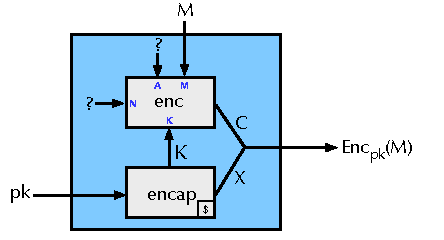
\includegraphics[scale=1.2]{kem-dem.pdf}
\caption{The motivating question: how to build (labeled) public-key encryption, via KEM-DEM, over an IV-based AEAD scheme and a conventional (randomized) KEM scheme.}
\label{fig:kem-example}
\end{center}
\end{figure}

The first is to demand that the KEM-scheme produces an appropriate IV.  One way to handle this is to define a new type of KEM primitive that includes an algorithm for creating IVs, along with the usual encapsulation and decapsulation algorithms.  Alternatively, we could define a new kind of encapulation algorithm that returns a triple $(K,X,\pubiv)$.  In this case, the algorithm~$\encap$ may need to be both randomized (for generation of~$K$) \emph{and} stateful, if~$\pubiv$ must be a nonce.  (If the underlying AEAD scheme remains secure when~$\pubiv$ is a nonce only with high probability, then $\encap$ need not be stateful.)  Either way, the public-key encryption scheme that results from the KEM-DEM construction remains randomized.  See the left panel of Figure~\ref{fig:kem-dem options} for a psuedocode description of this construction.  Note that we must send~$\pubiv$ as part of the ciphertext (in order to make decrpytion possible), and we choose not to require that~$\pubiv$ be recoverable from~$X$, in order to cleanly separate the encapsulated secret key~$K$ from the public IV.

Although some syntactic changes are required to the standard KEM formalism, it seems unlikely that this option will provide any surprises.  As long as the encapsulation scheme generates~$\pubiv$ in a way that is appropriate for the underlying symmetric AEAD scheme, security statements for the KEM-DEM construction should be straightforward.

\begin{figure}
\begin{center}
\hfpagesss{.25}{.25}{.25}
{
\underline{$\Encprim{\pk}{}{\header, M}$}:\\[2pt]
$(K,X,\pubiv) \getsr \encap_\pk()$\\
$C \gets \encprim{K}{}{\header,\pubiv,M}$\\
Return $(X,N,C)$

\medskip
\underline{$\Decprim{\sk}{}{\header,X,N,C}$}:\\[2pt]
$K \gets \decap_\sk(X)$\\
$M \gets \decprim{K}{}{\header,\pubiv,C}$\\
Return $M$
}
{
\underline{$\Encprim{\pk}{}{\header,\pubiv,M}$}:\\[2pt]
$(K,X) \getsr \encap_\pk()$\\
$C \gets \encprim{K}{}{\header,\pubiv,M}$\\
Return $(X,C)$

\medskip
\underline{$\Decprim{\sk}{}{\header,\pubiv,X,C}$}:\\[2pt]
$K \gets \decap_\sk(X)$\\
$M \gets \decprim{K}{}{\header,\pubiv,C}$\\
Return $M$

}
{
\underline{$\Encprim{\pk}{}{\header,\pubiv,\seciv,M}$}:\\[2pt]
$(K,X) \gets \encap_{\pk}(\header,\pubiv,\seciv)$\\
$C \gets \encprim{K}{}{\header,\pubiv,M}$\\
Return $(X,C)$

\medskip
\underline{$\Decprim{\sk}{}{\header,\pubiv,X,C}$}:\\[2pt]
$K \gets \decap_\sk(X)$\\
$M \gets \decprim{K}{}{\header,\pubiv,C}$\\
Return $M$
}
\caption{KEM-DEM constructions using an symmetric-key IV-based AEAD scheme $(\enc,\dec)$. \textbf{Left:} Randomized or stateful scheme, in which the encapsulation algorithm generates the IV.  \textbf{Center:} Randomized scheme, in which the IV is surfaced.  \textbf{Right:} Deterministic scheme, in which the externally provided IV is separated into public and private components. The leftmost and rightmost schemes require new syntax for the encapsulation (and decapsulation) algorithms.}
\label{fig:kem-dem options}
\end{center}
\end{figure}


\paragraph{IV-based KEM-DEMs. }
A second option is to follow the what has been done in the symmetric setting, and surface the IV (and the associated data) as inputs to the KEM-DEM construction; see the center panel of Figure~\ref{fig:kem-dem options}.  
This shifts the requirements for IV generation to the calling environment, and unburdens the encapsulation algorithm~$\encap$.  We call any scheme that explicitly takes an IV as input \emph{IV-based}.  

The resulting IV-based public-key encryption scheme is still randomized, because $\encap$ is.  In some settings this may be appropriate.  For example, when the environment is not trusted to generate ---~and keep private~--- randomness for encapsulation, but can provide a reliable counter for the AEAD scheme.  \tsnote{What's a solid example of this?  HSMs accessed by many parties via a fixed API?  Cloud servers that don't know the clients and use TCP sequence number as counter}  In general, however, it seems cumbersome to have IV-based encryption that is also internally randomized.  
%And in applications in which the calling environment \emph{can} be trusted to generate a random IV for the underlying symmetric-key AEAD scheme, then it can provide randomness for other needs, too.
Thus, we consider a third option, that of building a \emph{deterministic} public-key encryption scheme via a KEM-DEM construction over a \emph{deterministic} KEM and an IV-based symmetric-key AEAD scheme.  See the right panel of Figure~\ref{fig:kem-dem options} for details.  

When the KEM-DEM scheme is made deterministic, no reasonable security seems achievable when the all inputs are known by the adversary.  So for our fully deterministic construction, we separate the IV into public and secret components $(\pubiv,\seciv)$.   
Note that we do not necessarilly demand that~$S$ be uniformly random, or that it be recoverable upon decryption.  However, we will require that $(N,S)$ be non-repeating and have a reasonable amount of min-entropy, and that~$S$ be treated as private data.  For example, $N$~might be a counter, and~$S$ a password.  We will see simple constructions in the random-oracle model in which this will suffice. As expected, the security of the construction will depend on the min-entropy in $(N,S)$. \tsnote{Standard-model instantiations, in which encapsulation uses a randomness extractor? There may be a chicken-and-egg problem with the extractor key, although maybe this can be published as part of the public-key for the scheme.}

\paragraph{Syntactic and security requirements on encapsulation. }  The first and last options require obvious syntatic changes to KEM-scheme syntax, as shown in Figure~\ref{fig:kem-dem options}. The deterministic option will also require new security notions for KEM schemes; in particular, a kind of nonce-based KEM security will be needed.  Informally, we will require that the output $(K,X)\gets\encap_{\pk}(A,N,S)$ be indistinguishable from $(R,X)$ where~$R$ is a uniform key for the underlying symmetric AEAD scheme.  This will be required only for adversaries that respect some min-entropy bound on the distribution of $(N,S)$. \tsnote{Not sure how the single-query vs.\ multiple-query issue plays out here.  Seems like you should be able to to have~$S$ be a single password that is used with multiple nonces~$N$ during a session.}

\paragraph{Prior work on PKE with associated data. } \tsnote{Definitely some work to consider.  Start with Shoup's paper: \texttt{http://www.shoup.net/papers/kdm-cca2.pdf}.  What problems has labeled PKE been used to solve?}

\paragraph{Prior work on deterministic PKE. } \tsnote{Which prior deterministic PKE schemes can be seen as examples or special cases of this new primitive? Lots of work in this area over the past 5-7 years. Security notions will likely be different, as we can allow the adversary to have the public key throughout the experiment, and there are nonces.}

\paragraph{Prior work on IV-based/deterministic KEM schemes. } \tsnote{I don't know if anyone has considered deterministic KEMs, but I'm guessing that this is a new primitive, too.  KEMs with associated data (``labels'') have been considered.  See H.\ Krawczyk, K.\ G.\ Paterson, and H.\ Wee, ``On the security of the TLS protocol: A systematic analysis'' and J.\ Jonsson and B.\ S.\ Kaliski. ``On the security of RSA encryption in TLS''}

\paragraph{Prior work on password-based encryption. } \tsnote{I don't know the password-based encryption literature very well.  Start with Bellare, Ristenpart, Tessaro and work backwards.}

\paragraph{Applications. } \tsnote{This is a big question! Nonce could be used by server to prevent replay attacks, and password provides a way to do client authentication(?)}

\section{Preliminaries}
\label{sec:prelims}
We begin with basic notation.  When $X,Y$ are bitstrings, we write $X \concat Y$ for their concatenation, $|X|$ for the bitlength, and $X\xor Y$ for their bitwise exclusive-or.  When $\calX$ is a set, we write $x \getsr \calX$ to mean that a value is sampled from $\calX$ and assigned to the variable~$x$.  Unless otherwise specified, sampling from sets is via the uniform distribution.

When~$F$ is an randomized algorithm, we write $x \getsr F(y_1,y_2,\cdots)$ to mean that~$F$ is run with the specified inputs and the result assigned to~$x$.  When~$F$ is determinsitic, we drop the $\$$-embellishment from the assignment arrow.  Algorithms may be provided access to one or more \emph{oracles}, and we write these as superscripts, e.g. $F^{\mathcal{O}}$; oracle access is black box and via an specified interface.  

An \emph{adversary} is a randomized algorithm.

\paragraph{Asymmetric (Public-key) Encryption Schemes. }
Fix sets $\pubkeys, \seckeys, \adata, \pubivs, \secivs, \ptxts, \ctxts$, the first two of which are nonempty.  An encryption scheme $\Pi=(\Kgen,\Enc,\Dec)$ is a triple of algorithms.  The randomized \emph{key generation} algorithm~$\Kgen$ takes no input and returns a public-key, secret-key pair $(\pk,\sk)$.  We write $(\pk,\sk)\getsr\Kgen$ for the operation of key generation.

The \emph{encryption} algorithm $\Enc \colon \pubkeys \times \adata \times \pubivs \times \secivs \times \ptxts \to \ctxts$ takes a public-key~$\pk\in\pubkeys$, associated data~$\header \in \adata$, public-IV~$\pubiv \in \pubivs$, secret-IV~$\seciv \in \secivs$ and a plaintext~$M \in \ptxts$, and returns a ciphertext~$C \in \ctxts$. 
When $\secivs$ is empty, then encryption is randomized.  Otherwise, it is \emph{IV-based} and deteministic.
To stress the differing semantics of the inputs, key and non-private/private data, we write $\Encprim{\pk}{\header,\pubiv}{S,M}$ instead of $\Enc(\pk,\header,\pubiv,\seciv,M)$ for the operation of encryption.  When encryption takes an oracle, we $\EncprimO{\pk}{\header,\pubiv}{\seciv,M}{\mathcal{O}}$ to clearly separate oracles from inputs.

The deterministic \emph{decryption} algorithm $\Dec \colon \seckeys \times \adata \times \pubivs \times \ctxts \to \left(\secivs \times \ptxts\right) \cup \{\bot\}$ takes a secret-key~$\sk\in\seckeys$, associated data~$\header \in \adata$, public-IV~$\pubiv \in \pubivs$, and a ciphertext~$C \in \ctxts$, and returns a pair $(S,M) \in \secivs\times\ptxts$, or the distinguished symbol~$\bot \not\in \ptxts$.  We write $(S,M) \gets \Decprim{\sk}{\header,\pubiv}{C}$ for the operation of decrpytion. 

For proper operation, we require that for all $(\pk,\sk)\in\pubkeys\times\seckeys$, $\header\in\adata$, $\pubiv\in\pubivs$, $\seciv\in\secivs$, and $M\in\ptxts$, we have $\Decprim{\sk}{\header,\pubiv}{\Encprim{\pk}{\header,\pubiv}{S,M}}=M$.

\paragraph{Symmetric Encryption Schemes. } [Fill in similarly, may ultimately consolidate.]

\paragraph{Encapsulation schemes. }
Let $\pubkeys, \seckeys, \adata, \pubivs, \secivs$ be as above, and let $\keys,\wraps$ be a nonempty sets.
%
An encapsulation scheme is a triple $(\pkgen,\encap,\decap)$.   The randomized \emph{key generation} algorithm~$\pkgen$ takes no input and returns a public-key, secret-key pair $(\pk,\sk)$.  We write $(\pk,\sk)\getsr\pkgen$ for the operation of key generation. 

The encapsulation algorithm $\encap \colon \pubkeys \times \adata \times \pubivs \times \secivs \to \keys \times \wraps$ takes a public-key~$\pk\in\pubkeys$, associated data~$\header \in \adata$, public-IV~$\pubiv \in \pubivs$, secret-IV~$\seciv \in \secivs$, and returns a key $K \in \keys$ and an encapsulation $X \in \wraps$. 
When $\secivs$ is empty, then the encapsulation algorithm is randomized.  Otherwise, it is \emph{IV-based} and deteministic.  Following our notational conventions, we write $\encapprim{\pk}{\header,\pubiv}{S}$ for the operation of encapsulation, and $\encapprimO{\pk}{\header,\pubiv}{\seciv}{\mathcal{O}}$ when it takes an oracle.  When one or more of $\header,\pubiv,\seciv$ is absent, it will be clear from context (rather than position) what inputs are present.

The decapsulation algorithm $\decap \colon \seckeys \times \wraps \to \keys \cup \{\bot\}$ takes a secret-key~$\sk\in\seckeys$ and an encapsulation $X \in \wraps$, and returns a key $K \in \keys$, or the distinguished symbol~$\bot \not\in \keys$.  We write $K \gets \decap_{\sk}(X)$ for the operation of decapsulation. 

For proper operation, we require that for all $(\pk,\sk)\in\pubkeys\times\seckeys$, $\header\in\adata$, $\pubiv\in\pubivs$, $\seciv\in\secivs$, if $\encap_{\pk}(\header,\pubiv,\seciv)$ returns $(K,X)$, then $\decap_{\sk}(X)=K$.

Our formalization of encapsulation schemes is a bit non-standard, as it allows encapsulation to take IVs and associated data.

\section{Security Notions}
\label{sec:notions}
\begin{figure}
\begin{center}
\fpage{.5}{
 \hpagess{.425}{.55}{
 \underline{$\ExpINDCDA{\pkscheme,\advD}{\advA}$}:\\[2pt]
 $(\pk,\sk)\getsr\Kgen$\\
 $b\getsr\bits$\\
 $S\getsr\advD$\\
 $b'\getsr\advA^{\OEnc(\cdot,\cdot,\cdot,\cdot)}(\pk)$\\
 Return $[b'=b]$\\

\medskip
 \underline{$\ExpINDCDAR{\pkscheme,\advD}{\advA}$}:\\[2pt]
 $(\pk,\sk)\getsr\Kgen$\\
 $b\getsr\bits$\\
 $S\getsr\advD$\\
 $b'\getsr\advA^{\OEnc(\cdot,\cdot,\cdot)}(\pk)$\\
 Return $[b'=b]$

 }
 {
 \Oracle{$\OEnc(\header,\pubiv,M_0,M_1)$}:\\[2pt]
 Return $\encprim{\pk}{\header,\pubiv}{S,M_b}$\\[54pt]

\medskip
 \Oracle{$\OEnc(\header,M_0,M_1)$}:\\[2pt]
 $N \getsr \pubivs$\\
 $C \gets  \encprim{\pk}{\header,\pubiv}{S,M_b})$\\
 Return $(N,C)$

 }
}
\caption{\textbf{Above:} The IND-CDA notion for IV-based PK-AEAD scheme~$\pkscheme$
  when the secret-IV sampler is~$\advD$.  We assume~$\advA$ is
  nonce-respecting. \textbf{Below:} The IND-CDA-IV notion, in which
  the public-IV~$\pubiv$ is a per-message random value.}
\label{fig:ind-cda}
\end{center}
\end{figure}

\section{Constructions}
\label{sec:constructions}
We begin by giving a simple construction of an IV-based PK-AEAD scheme that provides privacy (only) in the random-oracle model. It works for any randomized encapsulation algorithm $\OLencapprim{\pk}{}$, replacing its internally generated randomness with the output of the random oracle.  For example, the standard El Gamal KEM where $K=g^{\overline{S}x}$ and $X=g^{\overline{S}}$, for a generator~$g$ and $(\pk,\sk)=(g^x,x)$.


\begin{figure}
\begin{center}
\fpage{.5}{
 \hpagess{.45}{.55}{
 \underline{$\Encprim{\pk}{\header,\pubiv}{\seciv,M}$}:\\[2pt]
 $\overline{\seciv} \gets H(\pk \concat \header \concat \pubiv \concat \seciv)$\\ 
 $(K,\wrap) \gets \encapprim{\pk}{\header,\pubiv}{\overline{\seciv}}$\\
 $C \gets \encprim{K}{\header,\pubiv}{M \concat \seciv}$\\
 Return $(\wrap,C)$
 }
 {
 \underline{$\Decprim{\sk}{\header,\pubiv}{\wrap,C}$}:\\[2pt]
 $K \gets \decapprim{\sk}{\header,\pubiv}{\wrap}$\\[3pt]
 if $\decprim{K}{\header,\pubiv}{C} = \bot$ then\\
 \hspace*{3ex} Return $\bot$\\
 $M \concat S \gets \decprim{K}{\header,\pubiv}{C}$\\
 Return $(\seciv, M)$\\
 }
}

\medskip
\hspace*{.5ex}\fpage{.5}{
 \hpagess{.45}{.55}{
 \underline{$\encapprim{\pk}{\header,\pubiv}{\overline{\seciv}}$}:\\[2pt]
 $(K,X) \gets \OLencapprim{\pk}{}{\overline{\seciv}}$\\
 Return $(K,X)$
 }
 {
 \underline{$\decapprim{\sk}{\header,\pubiv}{X}$}:\\[2pt]
 $K \gets \OLdecapprim{\sk}{}{X}$\\
 Return $K$
 } 
} 
\caption{An IV-based PK-AEAD scheme, built in the KEM-DEM style, that is secure in the random-oracle model for hash function~$H$. The unspecified encapsulation algorithm $\overline{\encap}$ can be any randomized algorithm with its internal randomness replaced by~$\overline{\seciv}$.
}
\label{fig:ro-kem-dem-construction}
\end{center}
\end{figure}



%This particular construction allows for recovery of~$\overline{S}$ upon decryption.  In turn, this allows a re-encryption authenticty check on the decapsulated key~$K$, in addition to any authenticity checks on the ciphertext~$C$ that the AEAD scheme imposes.  \tsnote{The auth check on~$K$ is indirect, and we'll need to nail down what properties of the AEAD scheme are needed.}  
%By having decryption return $M \concat \overline{S}$, we might enable higher-level checks.  For example, if the senders secret IV~$S$ has been previously stored receiver-side, or transmitted out-of-band.  
Note that the secret IV is not required to change across encryption calls, so $S=\mbox{password}$ and $M=\mbox{ptxt}\concat \mbox{hash}(\mbox{password}\concat\mbox{salt})$ may provide a way for higher-level applications to check authenticity of the user, assuming $\mbox{hash}(\mbox{password}\concat\mbox{salt})$ is already known receiver-side.
%\tsnote{Need to patch up PKE syntax and proper operation requirement, if decryption returns something other than the plaintext that was encrypted (or $\bot$)} 






\bibliography{biblio}

\ifnum\camready=0
\appendix
\fi



\end{document}







